% Document class, paper size, base font size
\documentclass[a4paper, 12pt]{article}

% Encoding
\usepackage[utf8]{inputenc}
\usepackage[T1]{fontenc}

% Prevent indentation of beginning of paragraphs
\setlength{\parindent}{0em}

% Space between paragraphs
\parskip 0.5em

% include PDFs
\usepackage{pdfpages}

% Title, authors and date
\title{Exercise 4: Scrum Basics}
\author{
  Kendra Birringer\\
  (1229372)\and
  Nader Cacace\\
  (1208115)\and
  Steffen Hanzlik\\
  (1207417)\and
  Marco Peluso\\
  (1228849)\and
  Svetozar Stojanovic\\
  (1262287)
}
\date{November 16, 2019}


% Begin actual document
\begin{document}

\maketitle
\newpage
\tableofcontents
\newpage

\section{Describe the motivation for the introduction of Agile software processes. What is the difference compared to the classical waterfall model?}

"The idea of Agile Software Processes is to use the available time and resources as efficiently as possible to deliver an as good as possible software product at the end."
\cite{thoma1}.

Compared to the classical waterfall model, Agile software processes are more dynamic. A higher throughput of build and test are possible, because more computational resources and tools are available and through a Object Oriented design, changes to the software get more efficient which decreases the costs.

It is better to correct mistakes in earlier stages, it is too risky to plan too much in advance because of dynamic environments and competition.


\section{What are the basic characteristics of Scrum and why is it called a “framework”?}

Scrum is an incremental framework, that is transparent, lightweight and iterative. 
Scrum is not very formal and stringent, it only defines roles and rules based on the Agile principles. \cite{agileprinciples}

Scrum always needs to be adapted to the project's particular needs and team composition.

\section{What are the roles in the Scrum framework? Explain their responsibilities.}

There are three roles in the Scrum framework:

1. Product Owner:

The Product Owner has a very critical role: She is responsible and accountable for the project's success. Ideally there should only be one Product Owner per Scrum team. He is the stakeholder's representative. 
The Product Owner is in charge of defining User Stories, the assignment of the project's priorities and also manages the Product Backlog. He should also shield the development team from outside interference and only the Product Owner has the authority to accept projects as "Done".
\bigskip


2. Scrum Master:

The person is ideally a certified Scrum Master and is very experienced in Agile software process models.
In contrast to the Product Owner, the Scrum Master is able to work with more than one team.
He is the guide and coach to the team members and ensures that agile principles are followed by the team
She removes obstacles, prevents outside interventions, creates an environment where the team can work efficiently and ensures good communication between all team members .
\bigskip    

3. Development Team:

The Development Team consists of 5 to 10 people which are ideally located at the same place. They are self-organizing and manage their own work. This means that no one (not even the Scrum Master) tells the Development Team how to turn Product Backlog into Increments of potentially releasable functionality; the resulting synergy optimizes the Development Team’s overall efficiency and effectiveness.
Development Teams are cross-functional, the team members have all the necessary skills to create a product Increment. 
The team is responsible for all aspects of the development,  like testing, architecture, operations, or business analysis and is accountable for the success of a Sprint. \cite{scrumguideteamdev}


\section{What is the Product Backlog and what is the Sprint Backlog?}

Product Backlog:

Represents a list of all desired work on the project (including external and
         internal requests), which is owned and prioritized (ordered) by the Product Owner. In order to support planning each backlog item contains a rough estimate to support planning. For estimating the items the product owner and the development team work together.
\newpage
Sprint Backlog:

The most important items from the Product Backlog are contained in the Sprint Backlog. The development team refines the Sprint Backlog by breaking items down into tasks which then can be estimated more accurately. Then the development team decides the order and which tasks should be finished by whom.

\section{How and when is the Sprint Backlog created?}
The whole Scrum Team discusses about the items from the Product Backlog with the highest priority and choose the most important items that need to be done in the next Sprint. \cite{thoma2}

\section{What is the usual duration of a Sprint?}
According to the answers given on the quiz, the duration of a Sprint should be "Short enough" to minimize the business risk and it should not take longer than a month but also be "short enough to be able to synchronize the development work with other business events".
\cite{scrumorg}

\section{What do the various roles do during a Sprint?}

1. Product Owner:

The Product Owner "shields the development team from outside interference", so that the development team can work during the Sprint without any other interruptions. \cite{thoma3}
\bigskip

2. The Scrum Master:

The Scrum Master helps the Development Team to work without interruptions and provides a good working environment. Furthermore he/she tries to build a good relationship between the team members. \cite{thoma3}
\bigskip

3. The Development Team:

"During the actual time boxed Sprint, the team members work on their assigned tasks to turn the Sprint Backlog items into “Done”." \cite{thoma3}

\section{What is the “Daily Scrum”?}

The Daily Scrum is a 15 minute time boxed stand up meeting. It takes place every day at the same time, so no planning is needed. It is obligatory for the development team. The Scrum Master does not need to participate, but has to make sure it takes place and does not exceed 15 minutes.

The aim of the meeting is sharing information by each team member answering the following questions:
\begin{itemize}
        \item What did you do yesterday?
        \item Did you encounter any problems?
        \item What are you planning to do today?
    \end{itemize}
    

\section{What are the requirements upon the product at the end of a Sprint? How can this be ensured?}

"The Increment is the sum of all the Product Backlog items completed during a Sprint and the value of the increments of all previous Sprints. At the end of a Sprint, the new Increment must be "Done," which means it must be in useable condition and meet the Scrum Team’s definition of "Done". An increment is a body of inspectable, done work that supports empiricism at the end of the Sprint. The increment is a step toward a vision or goal. The increment must be in useable condition regardless of whether the Product Owner decides to release it." \cite{scrumguide2}

\section{Learning Material}
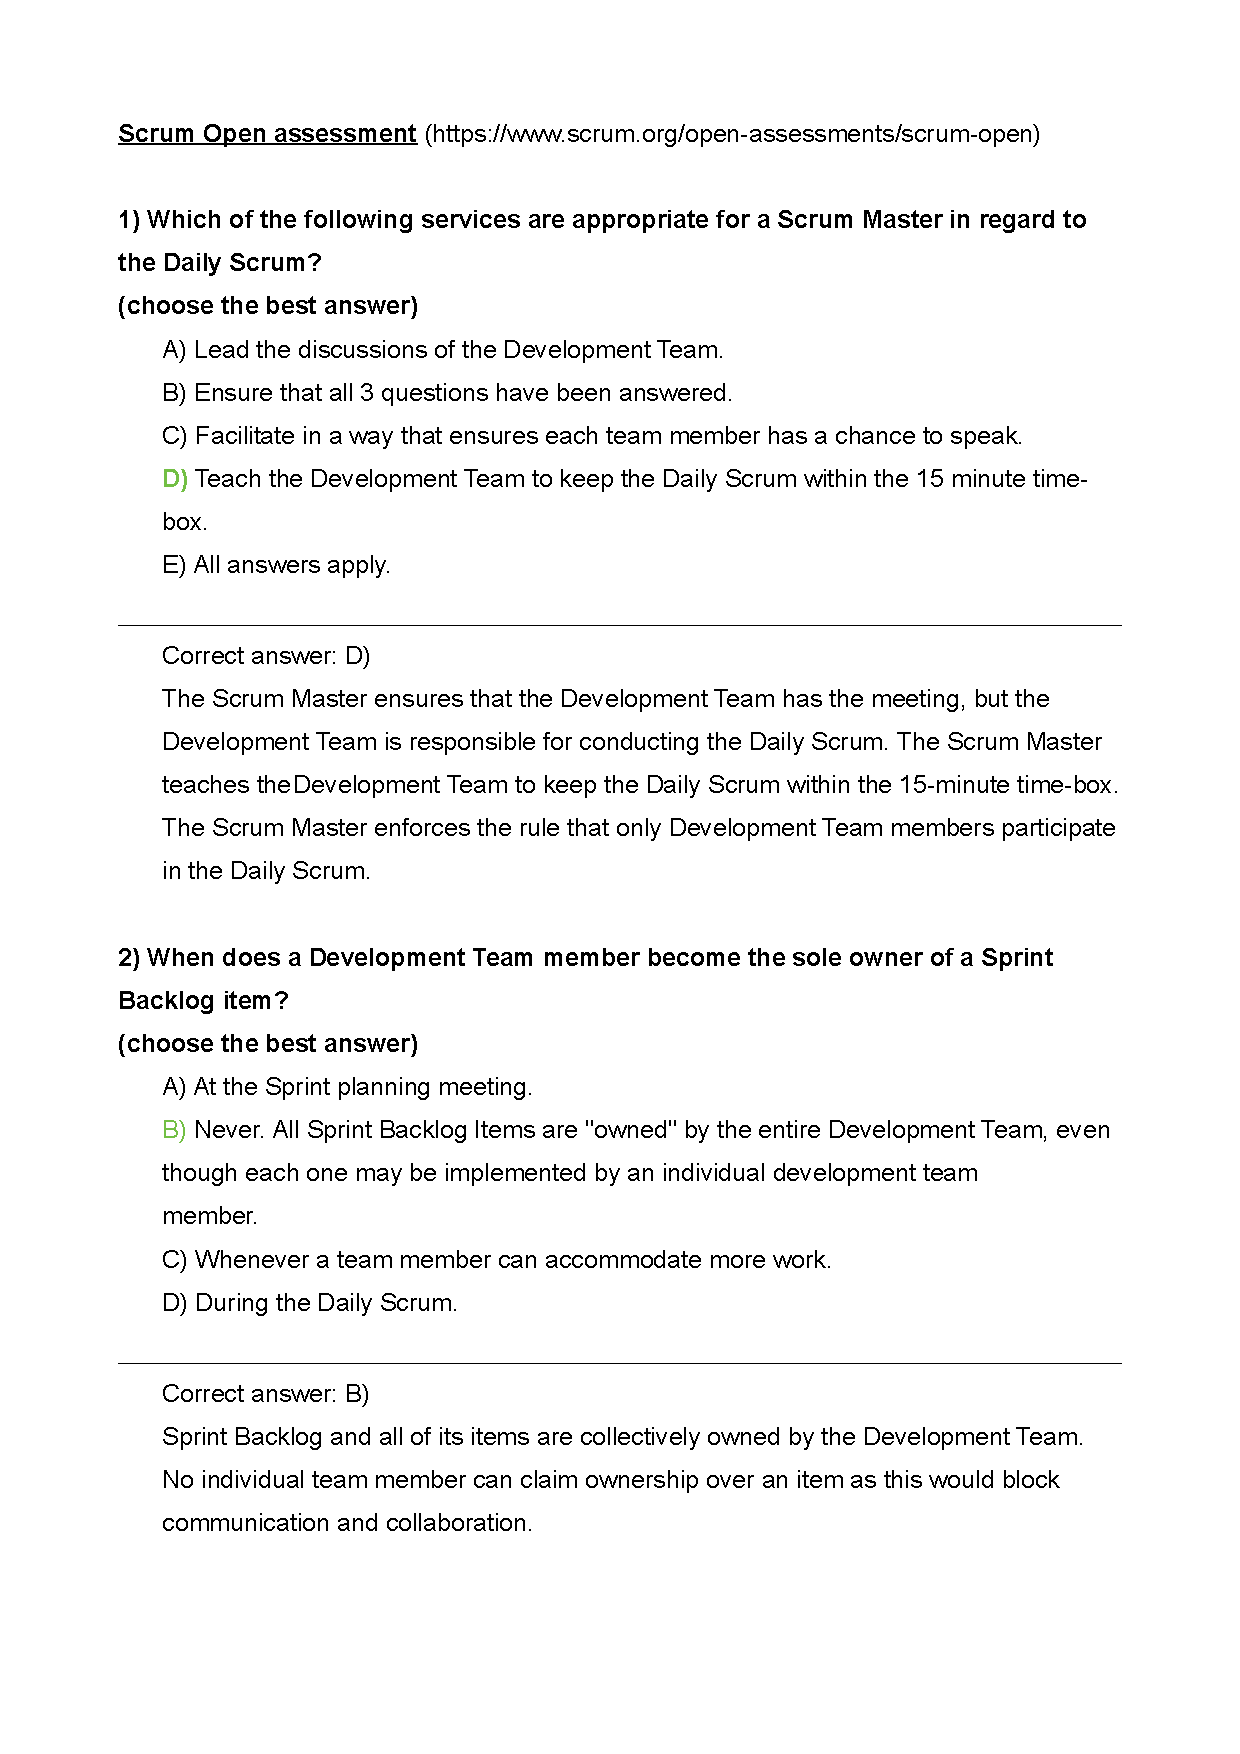
\includepdf[pages=-]{ScrumOpenAssessment.pdf}
\newpage

\section{Division of Work}
\renewcommand{\arraystretch}{1.5}
\begin{tabular}{|c|c|c|c|c|}
\hline
Kendra Birringer    & Nader Cacace  & Steffen Hanzlik   & Marco Peluso  & Svetozar Stojanovic\\
\hline
35\%                & 10\%          & 10\%              & 35\%          & 10\%\\
\hline
\end{tabular}
\newpage

\begin{thebibliography}{2}

\bibitem{thoma1}
Prof. Dr.-Ing Peter Thoma \emph{02-2 Software Engineering Analysis (Agile)}, 
slide 12, Winter-Semester 2019/2020

\bibitem{thoma2}
Prof. Dr.-Ing Peter Thoma \emph{02-2 Software Engineering Analysis (Agile)}

\bibitem{thoma3}
Prof. Dr.-Ing Peter Thoma \emph{02-3 Software Engineering Analysis (Scrum)}

\bibitem{agileprinciples}
https://www.agilealliance.org/agile101/12-principles-behind-the-agile-manifesto/

\bibitem{scrumguideteamdev}
https://www.scrumguides.org/scrum-guide.html\#team-dev

\bibitem{scrumguide2}
https://www.scrumguides.org/scrum-guide.html\#artifacts-increment

\bibitem{scrumorg}
https://www.scrum.org/open-assessments/scrum-open

\newpage
\end{thebibliography}

\end{document}
